% Redrawn figure 80/02-7 of the edition (transcripts/80/drawings/02-7.tex), copied for this article.
% Drawing 80/02-7 -- folder 80, batch 02, archive page 24 (PDF page 25).
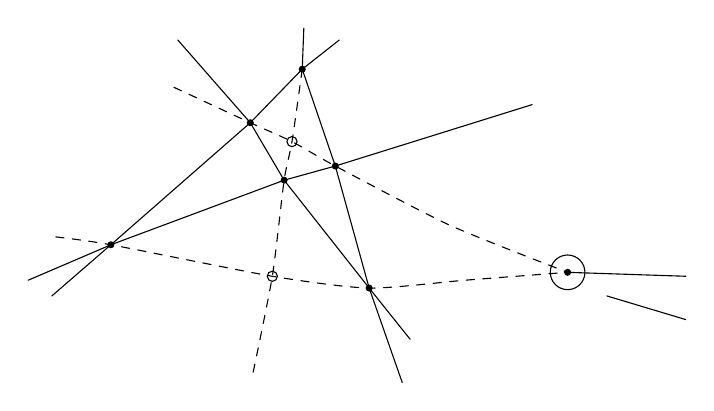
\begin{tikzpicture}[pencil/.style={black!45}, struck/.style={black!35}, mpt/.style={circle,draw,inner sep=1.3pt}, pt/.style={circle,fill,inner sep=0.9pt}, opt/.style={circle,draw,fill=white,inner sep=1.1pt},x=1mm,y=1mm,line cap=round,line join=round,font=\scriptsize]
\draw (7.5,-48) -- (15,-41.5) -- (32.7,-26) -- (39.3,-19.2) -- (44,-15.5);
\draw (4.5,-46) -- (15,-41.5) -- (37,-33.3) -- (43.5,-31.5) -- (68.5,-23.7);
\draw (23.5,-15.5) -- (32.7,-26) -- (37,-33.3) -- (47.8,-47) -- (53,-53.5);
\draw (39.5,-14) -- (39.3,-19.2) -- (43.5,-31.5) -- (47.8,-47) -- (52,-59);
\draw[dashed] plot[smooth, tension=0.4] coordinates {(23,-21.5) (32.7,-26) (38,-28.4) (43.5,-31.5) (58,-39) (73,-45)};
\draw (78,-48) -- (88,-51);
\draw[dashed] plot[smooth, tension=0.4] coordinates {(39.3,-19.2) (38,-28.4) (37,-33.3) (35.5,-45.5) (33,-58)};
\draw[dashed] plot[smooth, tension=0.4] coordinates {(8,-40.5) (15,-41.5) (35.5,-45.5) (47.8,-47) (60,-46) (73,-45)};
\draw (73,-45) -- (88,-45.5);
\node[pt] at (39.3,-19.2) {};
\node[pt] at (32.7,-26) {};
\node[pt] at (43.5,-31.5) {};
\node[pt] at (37,-33.3) {};
\node[pt] at (15,-41.5) {};
\node[pt] at (47.8,-47) {};
\node[pt] at (73,-45) {};
\node[mpt] at (38,-28.4) {};
\node[mpt] at (35.5,-45.5) {};
\draw (73,-45) circle[radius=2.2];
\end{tikzpicture}
